% Generated by Listas/make_statements.py from pratica-lecture-08.md, item 8. Do not edit.
\textbf{Source.} Muñoz-Garcia \& Toro-Gonzalez (2019), \emph{Strategy and Game Theory: Practice Exercises with Answers}, Ch. 9, Exercise 2 ``Job-Market Signaling Game'', pp.~385--386 {[}PDF pp.~394--395{]} (figure on p.~386). Reproduced verbatim (statement and its footnote 3 only; the book's worked answer follows it). Answer: yes, the book's worked answer follows the exercise.



\begin{quote}

Let us consider the sequential game with incomplete information depicted in Fig. 9.11. A worker privately observes whether he has a High productivity or a Low productivity, and then decides whether to acquire some education, such as a college degree, which he will subsequently be able to use as a signal about his innate productivity to potential employers. For simplicity, assume that education is not productivity enhancing. A firm that considers hiring the candidate, however, does not observe the real productivity of the worker, but only knows whether the worker decided to acquire a college education or not (the firm can observe whether the candidate has a valid degree). In this setting, the firm must respond hiring the worker as a manager (M) or as a cashier (C).³



\textbf{Part (a)} Does this game have an equilibrium using the strategy profile {[}NE'{]}



\textbf{Part (b)} Does this game have an equilibrium using the opposite separating strategy profile {[}EN'{]}



\textbf{Part (c)} Does this game have an equilibrium using the Pooling strategy profile {[}EE'{]} in which both types of workers acquire education.



\textbf{Part (d)} Does this game have an equilibrium using the pooling strategy profile {[}NN'{]}, in which neither type of worker acquires education.



\pandocbounded{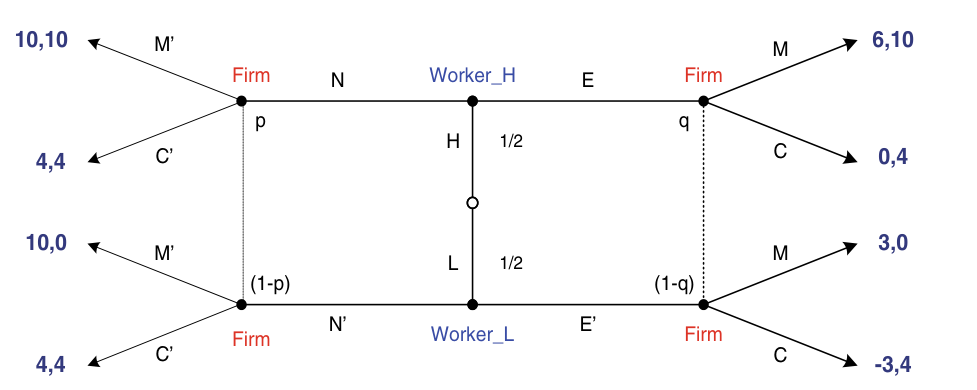
\includegraphics[keepaspectratio,alt={Fig. 9.11 The job-market signaling game}]{../figures/munoz-garcia-9-2.png}}



\emph{Fig. 9.11} The job-market signaling game



³This game presents a simplified version of Spence's (1973) labor market signaling game, where the worker can be of only two types (either high or low productivity), and the firm manager can only respond with two possible actions (either hiring the candidates as a manager, thus offering him a high salary, or as a cashier, at a lower salary). A richer version of this model, with a continuum of education levels and a continuum of salaries, is presented in the next chapter.

\end{quote}

